\chapter{Properties of Strontium}
\label{ap:SrProperties}

Appendix of (random) properties of strontium which may or may not all be used in this thesis. 

\section{Physical properties}

There are four naturally occurring stable isotopes of strontium: three bosons \Sr{88}, \Sr{86}, \Sr{84} with $I=0$ and a fermion \Sr{87} with $I=9/2$. 

\begin{table}[htbp]
	\centering
	\begin{tabular}{|c||c|c|c|c|}
		\hline
		Isotope	& $I$		& Statistics	& Natural abundance [\si{\percent}]	& Atomic mass [\si{\amu}]	\\	\hline	\hline
		\Sr{88}	& \num{0}	& Boson			& \num{82.58(1)}					& \num{87.9056125(12)}		\\	\hline
		\Sr{87}	& \num{9/2}	& Fermion		& \num{7.00(1)}						& \num{86.9088775(12)}		\\	\hline
		\Sr{86}	& \num{0}	& Boson			& \num{9.86(1)}						& \num{85.9092606(12)}		\\	\hline
		\Sr{84}	& \num{0}	& Boson			& \num{0.56(1)}						& \num{83.9134191(13)}		\\	\hline
	\end{tabular}
	\caption{\label{tab:sr_phys_prop}Physical properties of strontium \cite{nist_edi}.}
\end{table}

\section{Electronic properties}

\subsection{461 nm transition}

Transitions, detunings, scattering lengths, etc. 

\begin{table}[H]
\centering
\begin{tabular}{|l|l|l|l|l|}
\hline
Isotope 	& Lower level    				& Upper level 					& Frequency {[}kHz{]} 	& References 						\\ \hline
\Sr{88} 	& $\nSLJ{5s^2}{1}{S}{0}$ 		& $\nSLJ{5s5p}{1}{P}{1}$ 		&                     	& 						           	\\ \hline
\Sr{87} 	& $\nSLJF{5s^2}{1}{S}{0}{9/2}$ 	& $\nSLJF{5s5p}{1}{P}{1}{7/2}$ 	&                     	& 									\\
			& $\nSLJF{5s^2}{1}{S}{0}{9/2}$ 	& $\nSLJF{5s5p}{1}{P}{1}{9/2}$ 	&                     	& 									\\
			& $\nSLJF{5s^2}{1}{S}{0}{9/2}$ 	& $\nSLJF{5s5p}{1}{P}{1}{11/2}$ &                     	&									\\ \hline
\Sr{86} 	& $\nSLJ{5s^2}{1}{S}{0}$ 		& $\nSLJ{5s5p}{1}{P}{1}$ 		&                     	& 									\\ \hline
\Sr{84} 	& $\nSLJ{5s^2}{1}{S}{0}$ 		& $\nSLJ{5s5p}{1}{P}{1}$ 		&                     	&			 						\\ \hline
\end{tabular}
\caption{Isotopic transition frequencies of the 461 nm line.}
\label{blue_iso_freq}
\end{table}

\subsection{Strontium isotope shifts}

**Table for Sr isotope shifts?**

\subsection{689 nm transition}

\begin{table}[H]
\centering
\begin{tabular}{|c|c|c|l|}
\hline
Isotope						& Lower level									& Upper level										& \multicolumn{1}{c|}{Frequency [\si{kHz}]}							\\ \hline
\multirow{5}{*}{\Sr{88}}	& \multirow{5}{*}{$\nSLJ{5s^2}{1}{S}{0}$}		& \multirow{5}{*}{$\nSLJ{5s5p}{3}{P}{1}$}			& \num{434829121311 +- 10} \cite{Sansonetti_2010, Ferrari_2003}		\\ %\cline{4-4}
							&												&													& \num{434829121300 +- 20} \cite{Courtillot_2005}					\\ %\cline{4-4}
							&												&													& \num{434829121312.334 +- 0.039} \cite{Ido_2005}					\\ %\cline{4-4}
							&												&													& \num{434829121313 +- 20} \cite{Hui_2015}							\\ \cline{4-4}
							&												&													& \num{434829121312.334 +- 0.039}									\\ \hline
\multirow{9}{*}{\Sr{87}}	& \multirow{3}{*}{$\nSLJF{5s^2}{1}{S}{0}{9/2}$}	& \multirow{3}{*}{$\nSLJF{5s5p}{3}{P}{1}{7/2}$}		& \num{434830473270 +- 55} \cite{Sansonetti_2010, Courtillot_2005}	\\ %\cline{4-4}
							&												&													& \num{434830473218 +- 55} \cite{Hui_2015}							\\ \cline{4-4}
							&												&													& \num{434830473244 +- 39}											\\ \cline{2-4}
							& \multirow{3}{*}{$\nSLJF{5s^2}{1}{S}{0}{9/2}$}	& \multirow{3}{*}{$\nSLJF{5s5p}{3}{P}{1}{9/2}$}		& \num{434829343010 +- 50} \cite{Sansonetti_2010, Courtillot_2005}	\\ %\cline{4-4}
							&												&													& \num{434829342986 +- 65} \cite{Hui_2015}							\\ \cline{4-4}
							&												&													& \num{434829343001 +- 40}											\\ \cline{2-4}
							& \multirow{3}{*}{$\nSLJF{5s^2}{1}{S}{0}{9/2}$}	& \multirow{3}{*}{$\nSLJF{5s5p}{3}{P}{1}{11/2}$}	& \num{434827879860 +-55} \cite{Sansonetti_2010, Courtillot_2005}	\\ %\cline{4-4}
							&												&													& \num{434827879826 +- 60} \cite{Hui_2015}							\\ \cline{4-4}
							&												&													& \num{434827879844 +- 41}											\\ \hline
\multirow{3}{*}{\Sr{86}}	& \multirow{3}{*}{$\nSLJ{5s^2}{1}{S}{0}$}		& \multirow{3}{*}{$\nSLJ{5s5p}{3}{P}{1}$}			& \num{434828957494 +- 10} \cite{Sansonetti_2010, Ferrari_2003}		\\ %\cline{4-4}
							&												&													& \num{434828957493 +- 25} \cite{Hui_2015}							\\ \cline{4-4}
							&												&													& \num{434828957493.9 +- 9.3}**										\\ \hline
\Sr{84}						& $\nSLJ{5s^2}{1}{S}{0}$						& $\nSLJ{5s5p}{3}{P}{1}$							& \num{434828769718 +- 111} \cite{Hui_2015}							\\ \hline
\end{tabular}
\caption{Absolute transition frequencies of the 689 nm intercombination line.}
\label{red_iso_freq}
\end{table}

\section{Properties of \Srion{87}{+}}

Compared to the simple structure of singly ionized boson, \Sr{87}'s nuclear spin meaning \Srion{87}{+} exhibits hyperfine structure. 
In particular, the coupling of the single valence electron to the $I=9/2$ nuclear spin splits the \nSLJ{5s}{2}{S}{1/2} ground state in to $F=4$ and $F=5$ components \cite{sff_1993}.

\begin{figure}[!htbp]
	\centering
	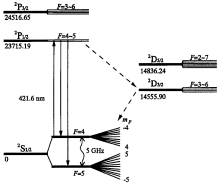
\includegraphics[width=8.6cm, keepaspectratio=true]{sff_1993-87Sr+.eps}
	\caption{Alkali-like energy levels of \Srion{87}{+}. Figure from \cite{sff_1993}.}
\end{figure}

From the measured hyperfine splittings, 